\documentclass[12pt]{article}
\usepackage[dvipsnames]{xcolor}
\usepackage{graphicx}
\usepackage{amsmath}
\usepackage{amssymb}
\usepackage[color,matrix,frame,arrow,curve]{xy}
\begin{document}


\begin{figure}[h!]\centering
\begin{minipage}{.5\linewidth}
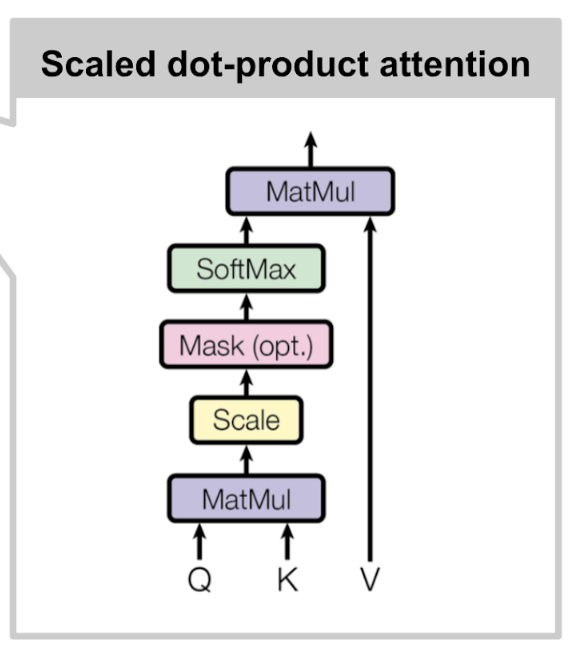
\includegraphics[width=2in]{scaled-dot-prod-att.jpg}
\end{minipage}%blank lines between minispaces breaks this
\begin{minipage}{.5\linewidth}
$$\xymatrix{
&&&*+[F*:Orchid]{\underline{P}^{3\times  4}}
\\
&*+[F*:SpringGreen]{\underline{G}^{3\times  4}}\ar[urr]&&
\\
&*+[F*:Lavender]{\underline{R}^{3\times  4}}\ar[u]&&
\\
&*+[F*:yellow]{\underline{Y}^{3\times  4}}\ar[u]&&
\\
&*+[F*:Orchid]{\underline{B}^{3\times  4}}\ar[u]&&
\\
*+[F*:Dandelion]{\underline{Q}^{3\times  4}}\ar[ur]&&*+[F*:Dandelion]{\underline{K}^{3\times  4}}\ar[ul]&*+[F*:Dandelion]{\underline{V}^{3\times  4}}\ar[uuuuu]
}$$
\end{minipage}
\caption{Scaled Dot Product Attention.}
\label{fig-texnn-for-scaled-dot-prod-att}
\end{figure}\begin{subequations}
\begin{equation}
Q^{3\times  4} =)
\label{eq-Q-fun-scaled-dot-prod-att}
\end{equation}

\begin{equation}
K^{3\times  4} =)
\label{eq-K-fun-scaled-dot-prod-att}
\end{equation}

\begin{equation}
V^{3\times  4} =)
\label{eq-V-fun-scaled-dot-prod-att}
\end{equation}

\begin{equation}
B^{3\times  4} = {\rm mat\_mult}(Q^{3\times  4},K^{3\times  4})
\label{eq-B-fun-scaled-dot-prod-att}
\end{equation}

\begin{equation}
Y^{3\times  4} = {\rm scale}(B^{3\times  4})
\label{eq-Y-fun-scaled-dot-prod-att}
\end{equation}

\begin{equation}
R^{3\times  4} = {\rm mask}(Y^{3\times  4})
\label{eq-R-fun-scaled-dot-prod-att}
\end{equation}

\begin{equation}
G^{3\times  4} = {\rm softmax}(R^{3\times  4})
\label{eq-G-fun-scaled-dot-prod-att}
\end{equation}

\begin{equation}
P^{3\times  4} = {\rm mat\_mult}(G^{3\times  4},V^{3\times  4})
\label{eq-P-fun-scaled-dot-prod-att}
\end{equation}

\end{subequations}


\end{document}  
